
\chapter{Hybrid Finite/Boundary Element Method}
\label{sec:hybr-finit-elem}
The hybrid finite/boundary element method works similarly to the normal finite element method except that one or more sub-regions are mapped onto their boundary \cite{Rammohan2002}.
The main advantage of this is that we reduce the dimensionality of these sub-regions one since we only have to solve equations on the boundary instead of the entire space.
In our case this is likely to give an advantage over a pure finite element method since we no longer need to mesh a long way outside the magnetic domain to accurately account for the effect of the external region. Also other methods for dealing with infinite domains can often give additional errors due to the truncation of the external domain.\cite{Bottauscio2008}

On the downside this mapping typically results in a dense matrix after discretisation, to which we cannot apply sparse matrix techniques.
Also the integrals that need to be computed may involve singularities, which introduce additional complications and may reduce accuracy or increase computation time.

Note that the derivation for this hybrid method comes from potential theory, rather than the boundary integral formulation usually used to construct the standard boundary element method.

\section{Background of the Method}
\label{sec:basic-method}
We want to use the boundary element method in the calculation of the magnetostatic scalar potential $\phim$, ($\hms = - \nabla \phim$), in the infinite region outside of a magnetic body.
Using the boundary element method directly, however, would require the solution of dense matrix equations for the entire problem.

We can circumvent this problem by splitting the potential into two parts $\phim = \phi_1 + \phi_2$ in such a way that $\phi_1$ can be calculated the magnetic region(s) using only the finite element method.
We then have some conditions on $\phi_2$ that must be satisfied to give the correct total potential in $\magd$ and on $\boundd$, but, in order to solve for $\phi_2$ in the magnetic domain, we still need to find the boundary conditions (on the edge of the magnetic domain).
So we choose a charge distribution on the boundary that satisfies all the conditions on $\phi_1$ and $\phi_2$.
We can then solve for $\phi_2$ on the boundary using similar techniques to those used in the boundary element method.
Finally we apply the finite element method to find $\phi_2$ inside the magnetic region $\magd$.

By the uniqueness of solution for Poisson's equation with Dirichlet and/or Neumann boundary conditions we know that the field $ \hms = \nabla \phim$  constructed by the above steps is \emph{the} magnetostatic field.\footnote{To see this take the difference of two solutions of Poisson's equation: $\phi = \psi_1 - \psi_2$. Then using identity \eqref{eq:20}, the linearity of Poisson's equation and the divergence theorem we obtain $\int_S \phi \nabla \phi \cdot d \mathbf{S} = \int_V (\nabla \phi)^2 dV$. Applying Dirichlet, Neumann or mixed boundary conditions shows that the boundary integral is zero and hence $\nabla \phi = 0$.}

\section{Problem Description}
\label{sec:problem-description}
Let $\phi^\inte$ be the value of $\phi$ (with subscripts as appropriate) close to the boundary $\boundd$ and just inside the magnetic domain  and $\phi^\exte$ the value of $\phi$ just outside the magnetic domain\footnote{More precisely $\phi^\inte(\xv) = \lim_{\xv \rightarrow \boundd} \phi(\xv)$ from inside the magnetic domain, $\phi^\exte(\xv) = \lim_{\xv \rightarrow \boundd} \phi(\xv)$ from outside the magnetic domain.} (see Figure~\ref{fig:BEM-geometry}).

We have the following \emph{physical} conditions\footnote{Equations~\eqref{eq:2}-\eqref{eqn:phibound} come from the definition of $\phi_m$, requirement for finite total energy, $\Bv^\text{int} \cdot \nv = \Bv^\text{ext} \cdot \nv$ and ??ds respectively.} on the total magnetostatic potential $\phim$:
\begin{equation}
  \lap \phim(\xv) = \nabla \cdot \mv(\xv) \qquad \forall \xv \in \magd \cup \extd,
  \label{eq:2}
\end{equation}
\begin{equation}
  \phim(\xv) \rightarrow 0 \qquad \text{ as } \abs{\xv} \rightarrow \infty,
\end{equation}
\begin{equation}
  \pd{\phim^\inte(\xv)}{\nv} - \pd{\phim^\exte(\xv)}{\nv} = \mv \cdot \nv \qquad \xv \in \boundd,
  \label{eqn:dphibound}
\end{equation}
\begin{equation}
  \phim^\inte(\xv) - \phim^\exte(\xv)  = 0 \qquad \xv \in \boundd.
  \label{eqn:phibound}
\end{equation}
Note that equations~\eqref{eqn:dphibound} and \eqref{eqn:phibound} imply continuity but not smoothness of the magnetic potential $\phim$ across $\boundd$. This is due to surface magnetic charges.

We choose $\phi_1$ to satisfy:
\begin{equation}
  \phim(\xv) = \phi_1(\xv) + \phi_2(\xv) \qquad \forall \xv \in \fulld,
  \label{eq:21}
\end{equation}
\begin{equation}
  \lap \phi_1(\xv) = \nabla \cdot \mv(\xv) \qquad \xv \in \magd,
  \label{eq:1}
\end{equation}
\begin{equation}
  \pd{\phi^\inte_1(\xv)}{\nv} = \mv \cdot \nv \qquad \xv \in \boundd,
  \label{eqn:dphionebound}
\end{equation}
\begin{equation}
  \phi_1(\xv) = 0 \qquad \xv \in \extd.
  \label{eqn:phioneoutside}
\end{equation}
Note that equations~\eqref{eq:1} and \eqref{eqn:dphionebound} give a self contained Poisson Neumann problem for $\phi_1 \in \magd \cup \boundd$.

The equations~\eqref{eq:2} to \eqref{eqn:phibound} for $\phim$ combined with equations~\eqref{eq:21} to \eqref{eqn:phioneoutside} for $\phi_1$ give a number of conditions on $\phi_2$ must satisfy. Since the Laplacian operator is linear, \ie $\lap \phim = \lap \phi_1 + \lap \phi_2$, from \eqref{eq:2} and \eqref{eq:1} it follows that
\begin{equation}
  \label{eq:8}
  \lap \phi_2(\xv) = 0 \qquad \forall \xv \in \fulld.
\end{equation}

Equation~\eqref{eqn:phioneoutside} implies that $\pd{\phi^\exte_1(\xv)}{\nv} = 0$. Combining this with equations (\ref{eqn:dphionebound}) and (\ref{eqn:dphibound}) gives
\begin{equation}
  \label{eq:5}
  \pd{\phi^\inte_2(\xv)}{\nv} - \pd{\phi^\exte_2(\xv)}{\nv} = 0.
\end{equation}

Finally from equations (\ref{eqn:phibound}), \eqref{eq:21} and (\ref{eqn:phioneoutside}) we have
\begin{equation*}
  \phi^\inte_1 - \phi^\exte_1 + \phi^\inte_2 - \phi^\exte_2 = 0,
\end{equation*}
\begin{equation}
  \phi^\inte_2 - \phi^\exte_2 = - \phi^\inte_1.
\label{eq:4}
\end{equation}

\begin{figure}
  \center
  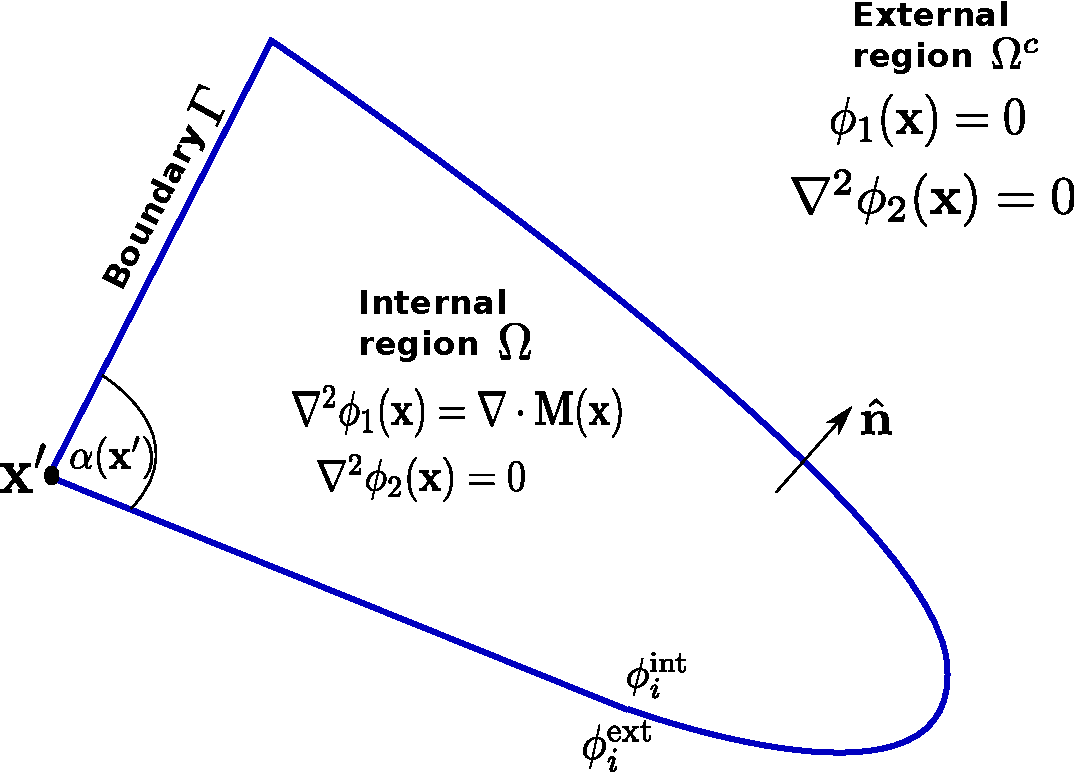
\includegraphics[width=0.75\textwidth]{./images/BEM-geometry}
  % \begin{tikzpicture}

  %   % Main nodes and some labels
  %   \node[label=below:$\xv'$] (a) at (-2,-2) {};
  %   \node (b) at (-2,2) {};
  %   \node[label=right:\Large{$\boundd$}] (c) at (5,0) {};

  %   % Draw main shape of magnetic domain
  %   \draw [line width=0.5mm,draw=solidblue,fill=paleblue] (a.north) to [bend right=71] (c) to (b.south);
  %   \draw [line width=0.5mm,draw=solidblue] (a) to (b);
  %   \draw (a.north) circle(1mm) [fill=black] {};

  %   % More labels
  %   \node (center) at (1,0) {\Large{Magnetic domain $\magd$}};
  %   \node(external) at (8,3) {\Large{External region $\extd$}};
  % \end{tikzpicture}

  \caption{A 2D representation of the geometry showing the labels used in this section. The point $\xv'$ is a singular point of the boundary $\boundd$, the angle $\alpha(\xv')$ is as shown.}
  \label{fig:BEM-geometry}
\end{figure}

\section{Double Layer Potentials}
\label{sec:double-layer-potent}
A double layer potential can be thought of as the potential due to a layer of dipoles of magnitude $\mu(\xv)$ in direction $\nv$ over the surface $S$.\cite{Sternberg1946} We will demonstrate that we can use a double layer potential to calculate $\phi^\inte_2$ in terms of $\phi^\inte_1$.

The double layer potential at a point $\xv \in \real^d$ is defined as \cite{eom_double_layer_potential}
\begin{equation}
  \label{eq:3}
  \phi(\xv) = \int_{S} \mu(\yv) \pd{\Green}{\nv} \d \yv,
\end{equation}
where $G$ is the Green's function for a Laplacian operator.
For $d=2$
\[ \Green = \dfrac{-1}{2\pi}\ln(\abs{\xv - \yv}), \]
and for $d=3$
\begin{equation} \Green = \dfrac{-1}{4 \pi} \dfrac{1}{\abs{\xv - \yv}}.
  \label{eqn:greenslaplacian3d}
\end{equation}


We have the following results from potential theory:\cite{Sternberg1946}
\begin{enumerate}
\item The double layer potential satisfies Laplace's equation $\lap \phi = 0$ (in other words the double layer potential is harmonic).% pages ?

\item The double layer potential undergoes a jump of $\mu(\xv)$ moving in the direction $\nv$ across a smooth surface $S$, \ie
  \begin{equation}
    \label{eq:15}
    \phi^\inte(\xv) - \phi^\exte(\xv) = \mu(\xv).
  \end{equation}
% pages 136-140

\item For $\xv \in S$ the following relationship holds
  \begin{equation}
    \phi^\inte(\xv) = (1 - \frac{\alpha(\xv)}{\alpha_{\text{max}}}) \mu(\xv) + \phi(\xv),
    \label{eq:22}
  \end{equation}
  where $\alpha(\xv)$ is the angle (or solid angle) in two (or three) dimensions subtended by the domain at $\xv$ and
\begin{equation*}
  \alpha_{\text{max}} =
  \begin{cases}
    2 \pi & \text{if } d=2 \\
    4 \pi & \text{if } d=3.
  \end{cases}\label{eq:16}
\end{equation*}
Note that $\alpha(\xv)$ is the angle at the exact point $\xv$, when the surface at $\xv$ is a Lyapunov surface (\ie not a sharp corner) $\frac{\alpha(\xv)}{\alpha_{\text{max}}}$ reduces to a factor of $1/2$. We write $\gamma(\xv) = \frac{\alpha(\xv)}{\alpha_{\text{max}}}$ for simplicity.
 % pages 137-139, page 155 for 2d

\item If $\mu$ is continuous and has continuous first and second derivatives along the boundary (\ie $\mu(\xv) \in C^2[S]$) then the limits $\pd{\phi^\inte(\xv)}{\nv}$ and $\pd{\phi^\exte(\xv)}{\nv}$ exist and are equal. % pages 145-153.

\end{enumerate}

Some notes on the derivation of the above results in Sternberg 1946\cite{Sternberg1946}:
\begin{itemize}
\item Some derivations of the results above rely on the surface being a ``Lyapunov surface'' which imposes a number of smoothness conditions, in particular excluding surfaces with corners.
The proofs given in Sternberg allow a finite number of sharp corners, \ie a polygonal domain.
\item Our potentials are a factor of $\frac{-1}{4 \pi}$ different from those in the reference. Also our $\phi^\inte$ and $\phi^\exte$ definitions correspond respectively to $\phi^-$ and $\phi^+$ in the book.
\end{itemize}

\section{Application to Magnetostatic Calculations}
From Section~\ref{sec:double-layer-potent} we can see that conditions \eqref{eq:8}, \eqref{eq:5} and \eqref{eq:4} on $\phi_2$ are satisfied by a double layer potential with magnitude
\begin{equation}
  \label{eq:24}
  \mu(\xv) = - \phi^\inte_1(\xv).
\end{equation}

By the uniqueness of solution for Poisson's equation this gives us, up to an additive constant, the only solution for $\phi_2(\xv)$ in the external region.
This is good enough for a potential since it is only used in $\hms(\xv) = - \nabla \phim(\xv)$ so addition of a constant has no effect.

From equations~\eqref{eq:3}, \eqref{eq:22} and \eqref{eq:24} we have:
\begin{equation}
  \label{eq:6}
  \phi^\inte_2(\xv) =  \big(\gamma(\xv) - 1 \big) \phi^\inte_1(\xv)
  - \int_{\boundd} \phi^\inte_1(\yv) \pd{\Green}{\nv} \d \yv.
\end{equation}
After substituting in our definition for the three dimensional Green's function \eqref{eqn:greenslaplacian3d} we obtain the same equation as given by Koehler \cite{Koehler1997}.
Similar equations are solved when using the standard boundary element method, hence the name.

Also note that $\phim = \phi_1 + \phi_2$ everywhere and so
\begin{align}
  \label{eq:18}
  \phim^\inte(\xv) &= \bm \big[ \phi^\inte_1(\xv) \big] \\
  &= \gamma(\xv) \phi^\inte_1(\xv)
  - \int_{\boundd} \phi^\inte_1(\yv) \pd{\Green}{\nv} \d \yv. \notag
\end{align}

Either equation~\eqref{eq:6} or \eqref{eq:18} can be used to give boundary conditions for $\phi_2 \in \magd$ or $\phim \in \magd$ respectively. We will proceed using equation~\eqref{eq:18} for simplicity since it eliminates $\phi_2$ from later calculations.

 Hence, given the solution for $\phi_1 \in \boundd$ (from solving \eqref{eq:1} and \eqref{eqn:dphionebound}) we have a complete Dirichlet Poisson problem for $\phim \in \magd \cup \boundd$:
\begin{align}
  \label{eq:phim-bem}
  \lap \phim(\xv) = \nabla \cdot \mv(\xv) \quad \xv \in \magd, \\
  \phim(\xv) = \bm \big[ \phi_1(\xv) \big] \quad \xv \in \boundd.
\end{align}

\section{Discretisation}
\label{sec:discretisation}

Given the operator $\bm$ the discretisation of equations~\eqref{eq:phim-bem}, \eqref{eq:1} and \eqref{eqn:dphionebound} is simple. We use standard finite elements as described in Section~\ref{sub:Actual-Finite-Elements}. We approximate $\phi^\inte_1$ and $\phi^\inte_2$ as the sum of a finite set of basis functions where each basis function corresponds a single node on the boundary $\boundd$. We will use test and shape functions identical except for boundary conditions to those used in Section~\ref{sec:spat-discr-resi}. So for $\phim$ the test functions are $\tbf_{\text{m}} \in \ts \cap \Dfs$, $\;\Dfs = \{ \tbf \st \tbf(\xv) \text{ satisfies the b.c. s } \; \forall \xv \in \boundd_D \}$. For $\phi_1$ they are $\tbf_1 \in \ts$ since we only have Neumann boundary conditions.

Hence the calculation of $\phi_1$ proceeds exactly as described in Section~\ref{sec:spat-discr-resi} with pure Neumann boundary conditions ($\boundd_\Neu = \boundd$ and $g_\Neu = \mv \cdot \nv$). Once we have the boundary conditions the calculation of $\phim$ proceeds similarly but with pure Dirichlet conditions ($\boundd_D = \boundd$). Therefore all that remains to be discretised is the operator $\bm$. We let
\begin{equation}
  \phim^\inte = \sum_\ibasis \phim_{,\ibasis}^\inte \tbf_{\text{m},\ibasis}(\xv),
  \qquad
  \phi^\inte_1 = \sum_\ibasisb \phi^\inte_{1,\ibasisb} \tbf_{1,\ibasisb}(\xv),
  \label{eq:25}
\end{equation}
where $\tbf_\ibasis(\xv_\ibasisb) = \delta_{\ibasis \ibasisb}$ on the boundary nodes and is linearly interpolated from $\tbf_\ibasis = 1$ at $\xv_\ibasis$ to $\tbf_\ibasis = 0$ at neighbouring nodes.

Substituting equations~\eqref{eq:25} into \eqref{eq:18} we have
\begin{equation*}
  \sum_\ibasis \phim_{,\ibasis}^\inte \tbf_{\text{m},\ibasis}(\xv) =
  - \int_{\boundd} \sum_\ibasisb \phi^\inte_{1,\ibasisb} \tbf_{1,\ibasisb}(\yv)
  \pd{\Green}{\nv} \d \yv
  \quad + \gamma(\xv) \sum_\ibasisb \phi^\inte_{1,\ibasisb} \tbf_{1,\ibasisb}(\xv).
\end{equation*}

To get the value of $\phim^\inte$ at node $\ibasisc$ we choose $\xv = \xv_\ibasisc$. Then using the property $\tbf_\ibasis(\xv_\ibasisc) = \delta_{\ibasis \ibasisc}$ and replacing $\ibasisc$ by $\ibasis$ we have
\begin{equation}
  \phim_{,\ibasis}^\inte =
  - \int_{\boundd_\ibasisb} \sum_\ibasisb \phi^\inte_{1,\ibasisb} \tbf_{1,\ibasisb}(\yv)
  \pd{\Green[\ibasis]}{\nv} \d \yv
  \quad + \gamma(\xv_\ibasis) \phi^\inte_{1,\ibasis},
  \label{eq:colocation}
\end{equation}
where ${\boundd_\ibasisb}$ is the region where $\tbf_{1,\ibasisb} \neq 0$, \ie the elements which contain node $\ibasisb$.

Finally, since the integrands are continuous functions ??ds citation needed, we can move the sum outside the integral leaving
\begin{equation}
  \phim_{,\ibasis}^\inte =
  - \sum_\ibasisb \phi^\inte_{1,\ibasisb} \Big[ \int_{\boundd_\ibasisb} \tbf_{1,\ibasisb}(\yv)
  \pd{\Green[\ibasis]}{\nv} \d \yv \Big]
  \quad + \gamma(\xv_\ibasis) \phi^\inte_{1,\ibasis}.
\label{eq:27}
\end{equation}
Notice that the expression inside the square brackets is independent of all the potentials: it depends only on the geometry and so can be pre-calculated and stored in many cases.

So equation~\eqref{eq:27} gives $\phim^\inte$ at a boundary node in terms of a sum of geometric factors multiplied by $\phi^\inte_1$ at each boundary node.
In other words, this is a dense matrix multiplication by a pre-computed matrix giving $\phim^\inte$ at all the boundary nodes in terms of $\phi^\inte_1$ at all boundary nodes:
\begin{equation}
  \label{eq:10}
  \phim_{,\ibasis}^\inte = \bm_{\ibasis,\ibasisb} \cdot \phi_{1,\ibasisb}^\inte,
\end{equation}
where
\begin{equation}
  \label{eq:17}
  \bm_{\ibasis\ibasisb} = - \int_{\boundd_\ibasisb} \tbf_{1,\ibasisb}(\yv) \pd{\Green[\ibasis]}{\nv} \d \yv
  \quad + \gamma(\xv_\ibasis)\delta_{\ibasis\ibasisb}.
\end{equation}


% ??ds wrong place for this discussion and not sure if integral is really singular or not due to the n.r term...
%Note that although this integral appears at first glance to be singular when the node $\xv_\ibasis$ is within $\boundd_\ibasisb$ (the line segment or section of surface being integrated over)
%A benefit of this is that the matrix is always well conditioned because the largest terms are near the singularity and hence near the diagonal elements $\ibasisb = \ibasis$.
%However the singularity can cause difficulties in the evaluation of the affected integrals.
%Methods to overcome these difficulties are discussed in the next section.

We now convert the normal derivative of the Green's function into a more tangible form.
In 3D
\begin{equation}
  \label{eq:11}
  \pd{\Green}{\nv} = \frac{-1}{4 \pi} \pd{}{\nv} \Gthreed = \frac{-1}{4 \pi} \nv \cdot \nabla \Big( \Gthreed \Big).
\end{equation}
Converting to spherical coordinates with the origin at $\xv_\ibasis$ ($r = \abs{\yv - \xv_\ibasis}$, $\ruv = \frac{\yv - \xv_\ibasis}{r}$) we have
\begin{equation}
  \label{eq:12}
  \pd{G(r)}{\nv} = \frac{-1}{4 \pi} \nv \cdot \ruv \pd{}{r} \Big( \frac{1}{r} \Big)
  = \frac{+1}{4 \pi}  \frac{\nv \cdot \ruv}{r^2}
  = \frac{\nv \cdot \rv}{4 \pi \abs{\rv}^3}
  ,\footnote{In spherical polar coordinates $\nabla = \ruv \pd{}{r} +  \phiv \frac{1}{r} \pd{}{\phi} + \thetav \frac{1}{r \sin \theta} \pd{}{\theta}$. Obviously $\frac{1}{r}$ has no angular dependence so only the derivative with respect to $r$ is non-zero.}
\end{equation}
\begin{equation}
  \label{eq:13}
  \pd{\Green}{\nv} = \frac{\nv \cdot \ruv}{4 \pi \abs{\yv - \xv_\ibasis} ^2} .
\end{equation}
Similarly in 2D we find
\begin{equation}
  \label{eq:14}
  \pd{\Green}{\nv} = \frac{-1}{2 \pi} \pd{}{\nv} (\Gtwod) = \frac{\nv \cdot \ruv}{2 \pi \abs{\yv - \xv_\ibasis}}.
\end{equation}

So the discretised boundary element matrix in $d=2,3$ dimensions is
\begin{equation}
  \label{eq:19}
  \bm_{\ibasis\ibasisb} =\frac{-1}{2^{(d-1)} \pi} \int_{\boundd_\ibasisb} \tbf_{1,\ibasisb}(\yv) \frac{\nv(\yv) \cdot \ruv_{\xv_{\ibasis} \rightarrow \yv}}{\abs{\yv - \xv_\ibasis} ^{d-1}} \d \yv
   \quad + \gamma(\xv_\ibasis)\delta_{\ibasisb\ibasis},
\end{equation}
where the subscript on $\ruv_{\xv_{\ibasis} \rightarrow \yv}$ is to remind us that the unit vector goes from $\xv_j$ to $\yv$.  We denote the integral in this equation by $I_\bm$.

\section{Discussion}

\subsection{Discretisation Approaches: Co-location vs Galerkin}

In deriving equation~\eqref{eq:colocation} we used a co-location approach rather than the Galerkin approach used in our FEM method.
The reason for this choice is that a Galerkin discretisation would lead to a double integral over the boundary, which would probably be more difficult to calculate.

Not sure what effect this has, if any, on the stability or accuracy of the scheme...


\subsection{The Matrix $\bm$}
Since $\bm$ is a dense matrix the processing and memeory requirements to compute, store and use $\bm$ scales as $\order{N_b^2}$ where $N_b$ is the number of boundary nodes. For some geometries (\eg nearly spherical objects) the overall computational complexity remains $\order{N}$ but for others (especially very thin films) the complexity can approach $\order{N^2}$.

It should be noted that $\bm$ depends only on the geometry of the problem and so typically only needs to be computed once, at the beginning of the simulation. Hence the integral computation time is not too important. Although if spatial adaptivity is used the geometry will change with every adaptation and $\bm$ will need to be recalculated.

One way to reduce the problems associated with the dense nature of $\bm$ is to use hierarchical matrix techniques. In this type of matrix the less important entries (\ie smaller) are lumped into a single entry similarly to multipole approximation methods. The cost of multiplication and storage of $\bm$ is thus reduced to only $\order{N \log(N)}$.\cite{Knittel2009}

\subsection{The Integral $I_\bm$}
Another factor that should be considered is the apparent singularity in the integral $I_\bm$ when integrating over an element containing the source point $\xv_\ibasis$. There are two distinct cases to look at here: flat elements and curvilinear elements.

In the case of flat elements if $\xv_\ibasisb$ is within the element being integrated over then we have
\begin{equation}
  \label{eq:7}
  \nv(\yv) \cdot \ruv_{\xv_{\ibasis} \rightarrow \yv} \equiv 0 \quad \forall \yv \in \text{element}.
\end{equation}
So the integral is zero and the singularity is avoided. Unfortunately for neighbouring elements this is not necessarily true--in particular elements at a sharp corner may be very close to a node where $\nv(\yv) \cdot \ruv_{\xv_{\ibasis} \rightarrow \yv} \neq 0$ resulting in a near-singular integral.

For curvilinear elements we no longer have the nice property that any potentially singular elements are automatically zero. However it can be shown that for reasonably shaped elements ??ds citation needed! there are still no real singular integrals only near-singular ones. This is due to the fact that $\nv(\yv) \cdot \ruv_{\xv_{\ibasis} \rightarrow \yv}$ tends to zero ``faster'' than $\abs{\yv - \xv_\ibasis}^2$ so the limit of the ratio as $\yv \rightarrow \xv_\ibasis$ is zero. In fact integrals like this are routinely evaluated in standard boundary element methods ??ds citation needed.

% \subsection{Corner Singularities}

% ??ds Think these are real...

% ??ds doesn't really go here...

% ??ds Rave, Thaville etc.


\section{Calculation of the integral $I_\bm$}

\subsection{Analytical solutions}

analytic formula given by.... for linear shape functions on triangles (implies flat element).

specifics of his shape functions

solution + notation

comments on references


\subsection{Numerical integration}

Advantages of numerical: flexible wrt to element shape

potentially allows higher order elements

potentially cheaper, at least for distance, non-near-singular elements



%%% Local Variables:
%%% mode: Latex
%%% TeX-master: "main"
%%% End:
